\documentclass[a4paper]{article}

\usepackage[english]{babel}

\usepackage[a4paper,top=2cm,bottom=2cm,left=3cm,right=3cm,marginparwidth=1.75cm]{geometry}

\usepackage[%
  titleformat=italic,% Titles in italic 
  titleformat=commasep,% A comma between athors and title 
  titleformat=all,% Always show a title (or a short title)
  commabeforerest,% A comma after title 
  ibidem=strict,% 
  citefull=first,% The first citing in full form 
  oxford,% The oxford style
  super,% Footnotes 
  dotafter=true,% 
  see,% An extra optional argument as a prenote 
  idem
]{jurabib}

\usepackage{amsmath}
\usepackage{graphicx}
\usepackage{bbold}

\title{Elliptic curves in modern cryptography}
\author{Andrei Lupsa}

\begin{document}
\maketitle

\begin{abstract}
Abstract!!
\end{abstract}


\section{Introduction to elliptic curves}

Formally, an elliptic curve is any implicit function where one variable has a degree of 2 and the other has a degree of 3. The kind we are interested in is elliptic curves in \textbf{short Weierstrass form}. This means they are in the form $y^2 = x^3 + ax^2 + b$. Examples of elliptic curves in short Weierstrass form can be seen in Figure \ref{fig:curves}.

\begin{figure}[h]
    \centering
    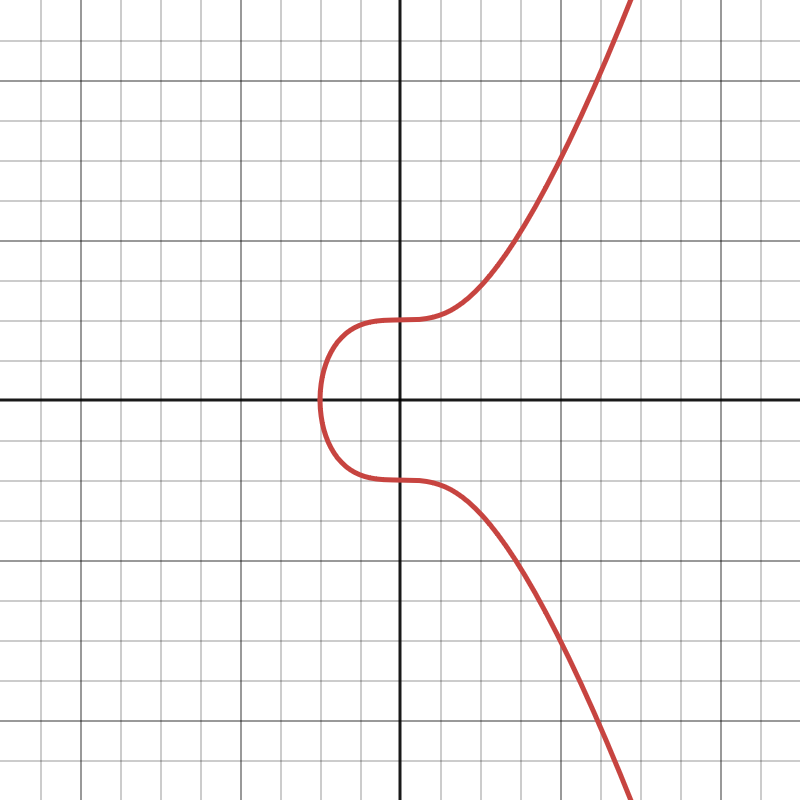
\includegraphics[width=0.2\linewidth]{images/curve-a0-b1.png}
    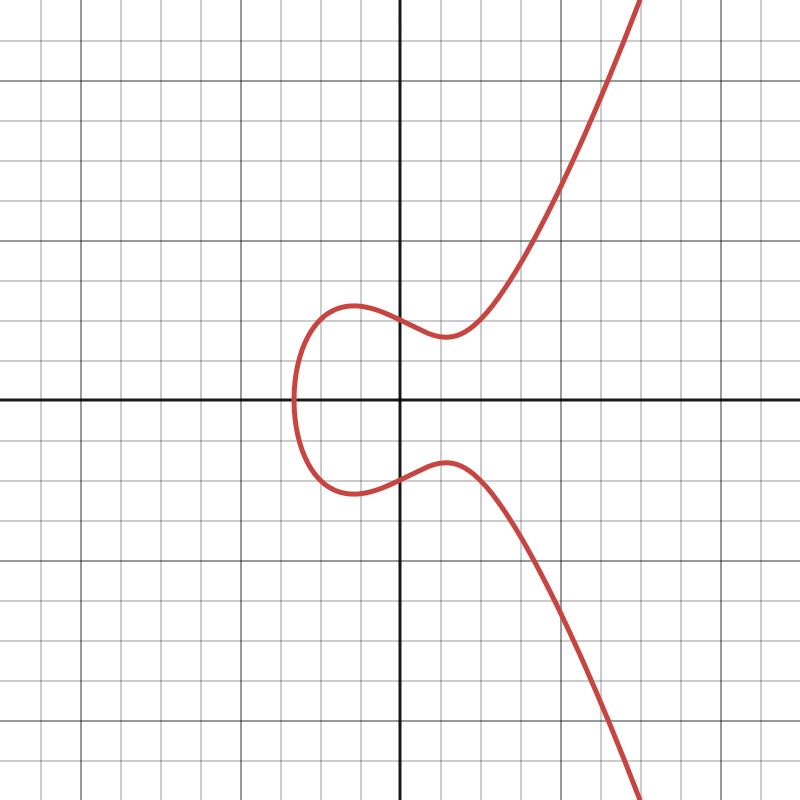
\includegraphics[width=0.2\linewidth]{images/curve-a-1-b1.png}
    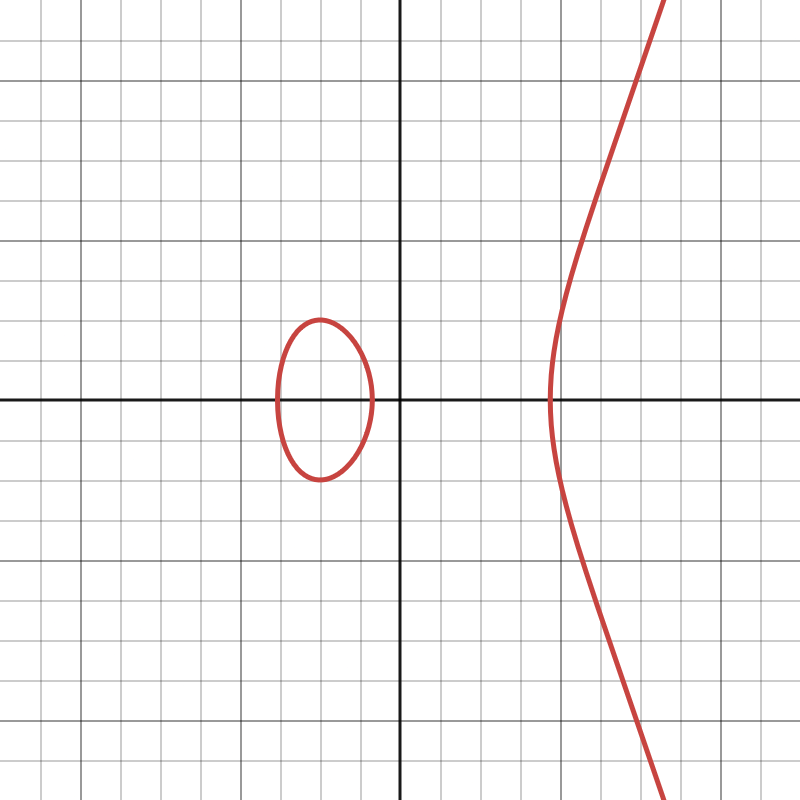
\includegraphics[width=0.2\linewidth]{images/curve-a-3-b-1.png}
    \caption{Several elliptic curves with different parameters.}
    \label{fig:curves}
\end{figure}


\section{Elliptic curve point arithmetic}

\subsection{Abelian groups}

An abelian group \textit{under a certain operation} is a group for which that operation is closed, commutative and associative, and for which there exists an inverse for every element and an identity element.\cite[p. 11]{wp}

A group $G$ that acts as an abelian group under an operation addition, $+$, is written as $(G, +)$. In other words, an abelian group $(G, +)$ has the following properties for all elements $A \in G$:
\begin{enumerate}
    \item \textbf{Commutativity.} $A + B = B + A$.
    \item \textbf{Associativity.} $(A + B) + C = A + (B + C)$.
    \item \textbf{Identity element.} There exists an element $I$ such that $A + I = I + A = A$.
    \item \textbf{Inverse elements.} There exists an inverse $A'$ for every element $A$ such that $A + A' = A' + A = I$.\cite[p. 11]{guide}
\end{enumerate}

An example of an abelian group is the integers under addition $(\mathbb{Z}, +)$, with the identity element $0$. 

An example of something that is \textit{not} an abelian group is the real numbers under multiplication $(\mathbb{R}, \times)$, because $0$ has no inverse. However, the real numbers excluding $0$ is an abelian group $(\mathbb{R} \setminus \{0\}, \times)$ with identity element $1$.

\subsection{Point addition \& doubling}

The points of an elliptic curve --- the pairings $(x,y)$ that satisfy the equation of the curve --- form an abelian group under an operation which we define as addition. 

Importantly, the addition of two points $(x_1, y_1) + (x_2, y_2) \ne (x_1 + x_2, y_1 + y_2)$; point addition is \textbf{not} vector addition. Rather, the addition of points on an elliptic curve is best illustrated graphically:

\begin{figure}[h]
    \centering
    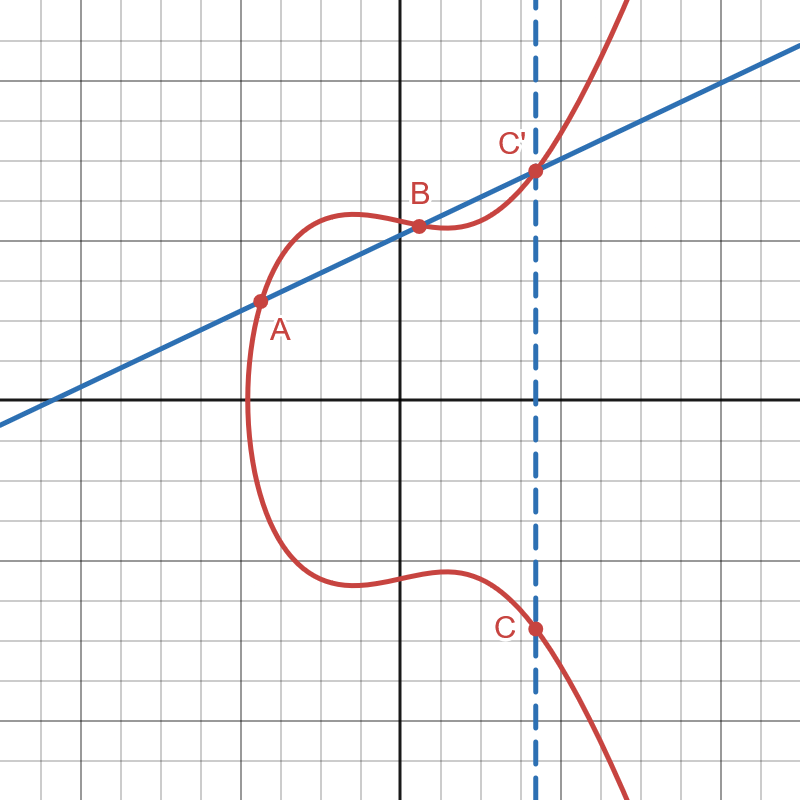
\includegraphics[width=0.3\linewidth]{images/add-add.png}
    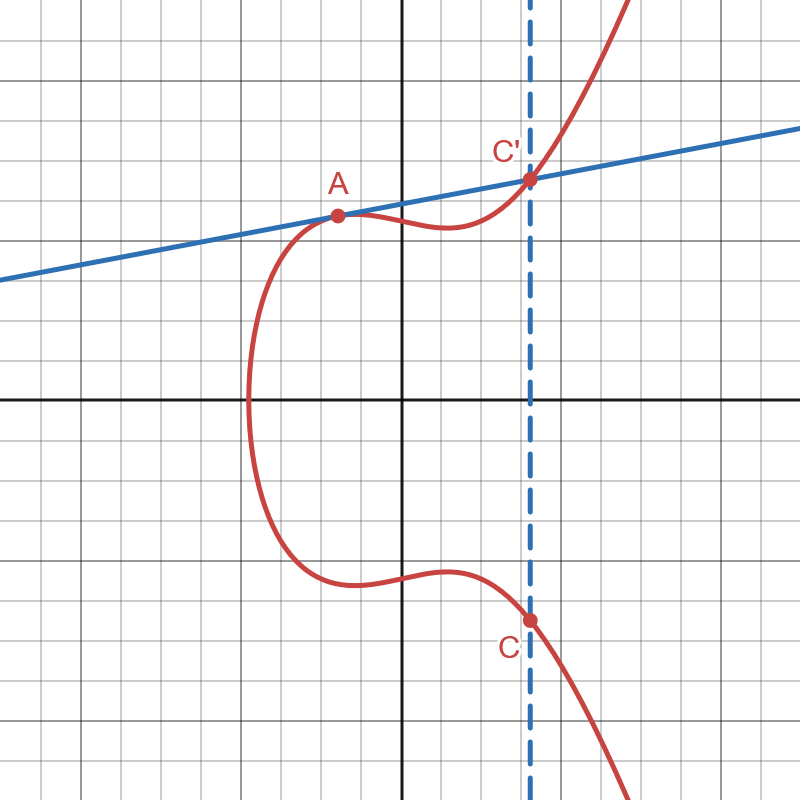
\includegraphics[width=0.3\linewidth]{images/add-double.png}
    \caption{Elliptic curve point addition and doubling..}
    \label{fig:add}
\end{figure}

To add two points $A$ and $B$: 
\begin{enumerate}
    \item Draw a line between the points $AB$.
    \item A line that intersects an elliptic curve at two points will \textit{always} intersect the curve at a third point (except for special cases, see Section \ref{poi} on the point at infinity).
    \item Take the third point and reflect it across the x-axis to obtain point $C$.
    \item $A + B = C$
\end{enumerate}

The process is similar for adding a point to itself (point doubling), where a line cannot be drawn between two points:
\begin{enumerate}
    \item Draw a line tangential to the curve at point A.
    \item The line will intersect the curve again at another point.
    \item Take the second point and reflect it across the x-axis to obtain point $C$.
    \item $A + A = C$
\end{enumerate}

Also important to note is that every point $A(x, y)$ has an inverse $A'(x, -y)$ in order to satisfy the properties of an abelian group. This property is used when defining the point at infinity (Section \ref{poi}).

\subsection{Derivation of point addition \& doubling equations}

Take two points on an elliptic curve $E$ where $A(x_1, y_1) + B(x_2, y_2) = C(x_3, y_3)$ . Let the line through $A$, $B$ and $C'(x_3, -y_3)$ be $L$ such that
\begin{gather*}
    E: y^2 = x^2 + ax + b \\
    L: y = \lambda x + m \\
    \text{where } \lambda = \frac{y_2-y_1}{x_2-x_1}
\end{gather*}

The intersection of $E$ and $L$ satisfies the equation
\begin{align*}
    x^3 + ax + b = (\lambda x + m)^2 \\
    x^3 + ax + b = \lambda^2 x^2 + 2 \lambda x m + m^2 \\
    x^3 - \lambda^2 x^2 + (a - 2 \lambda m)x + b - m^2 = 0
\end{align*}

We also know this equation has roots at $x_1$, $x_2$ and $x_3$, and can be written as
\begin{align*}
    (x-x_1)(x-x_2)(x-x_3)=0 \\
    x^3 - (x_1 + x_2 + x_3)x^2 + (x_1x_2 + x_1x_3 + x_2x_3)x - x_1x_2x_3 = 0
\end{align*}

Comparing coefficients of $x^2$ in the two forms of the equation, we can see that \[\lambda^2 = x_1 + x_2 + x_3\] and therefore \[x_3 = \lambda^2 - x_1 - x_2\] which gives the equation for $x_3$. To find $y_3$, we use the fact that $\lambda$ is also equal to the gradient between $C'(x_3, -y_3)$ and $B$:
\begin{align*}
    \lambda = \frac{-y_3-y_1}{x_3-x_1} \\
    -y_3 - y_1 = \lambda(x_3-x_1) \\
    y_3 = \lambda(x_1-x_3)-y_1
\end{align*}
and we have the equation for $y_3$.\cite{proof}

Adapting these equations for point doubling $A + A = C$ is easy; as the line is no longer through two points but rather the tangent at $A$, we differentiate $E$ to find the new gradient $\lambda$:
\begin{align*}
    y^2 = x^3 + ax + b \\
    2y\frac{dy}{dx} = 3x^2 + a \\
    \frac{dy}{dx} = \frac{3x^2 + a}{2y}
\end{align*}
and so \[\lambda = \frac{3x_1^2 + a}{2y_1}\]

Also, as $x_1 = x_2$, the equation for $x_3$ becomes \[x_3 = \lambda^2-2x_1\]

The equation for $y_3$ is unchanged.

\subsection{Point at infinity}\label{poi}

When the points of an elliptic curve are used as an abelian group $(G, +)$, we have to define an identity element. We call this identity element the \textit{point at infinity}, which is written as $\infty$, $\mathcal{O}$ or $0$. This is a point that lies on the curve which we imagine to be at $(\infty, \infty)$ and that satisfies the equations
\begin{enumerate}
    \item $A + \infty = \infty + A = A$
    \item $\infty + \infty = \infty$
\end{enumerate}

The point at infinity is the result of two operations:
\begin{enumerate}
    \item Adding a point to its own inverse, so $A + A' = \infty$.
    \item Doubling the point $A$ that is vertically tangential to the curve, where $2A = \infty$. This is because $A = A'$ for that point.
\end{enumerate}

\begin{figure}[h]
    \centering
    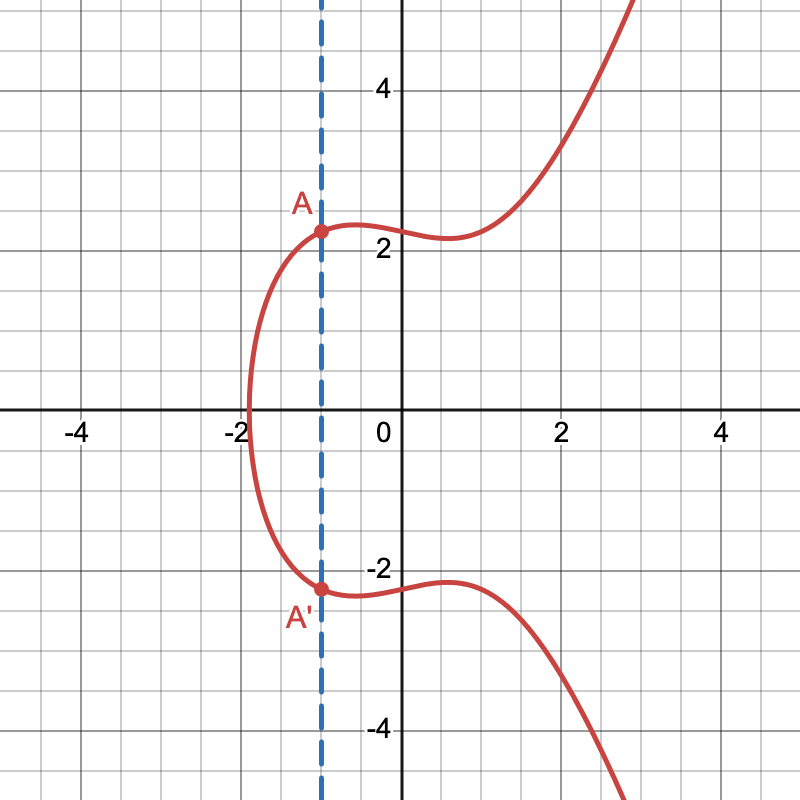
\includegraphics[width=0.3\linewidth]{images/infty-inverse.png}
    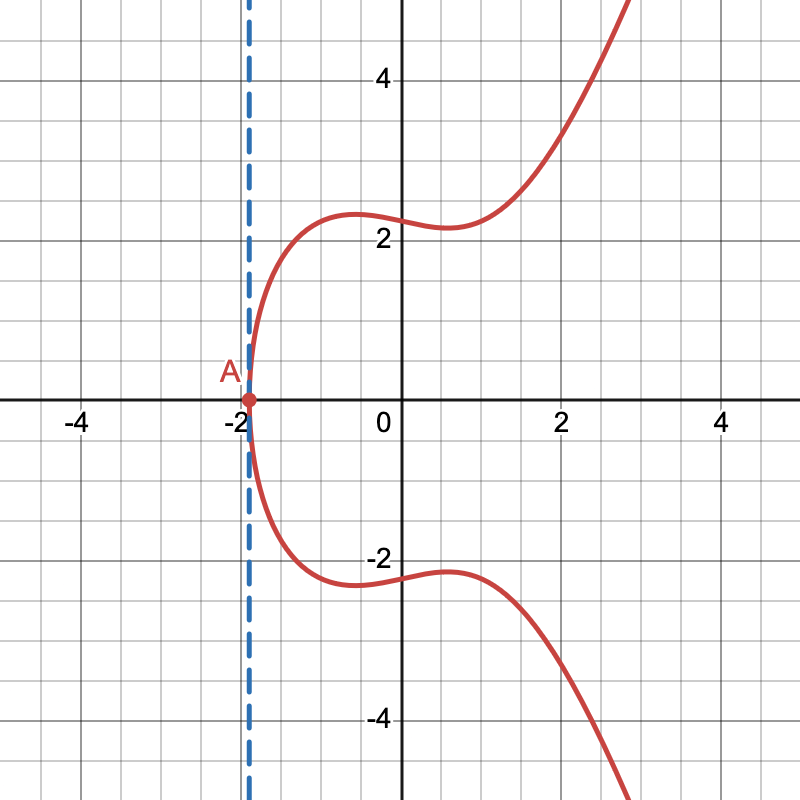
\includegraphics[width=0.3\linewidth]{images/infty-tangent.png}
    \caption{Two cases in which the point at infinity is produced.}
    \label{fig:infinity}
\end{figure}


\section{Elliptic curves over prime fields}

\subsection{Finite fields}

\begin{figure}[h]
    \centering
    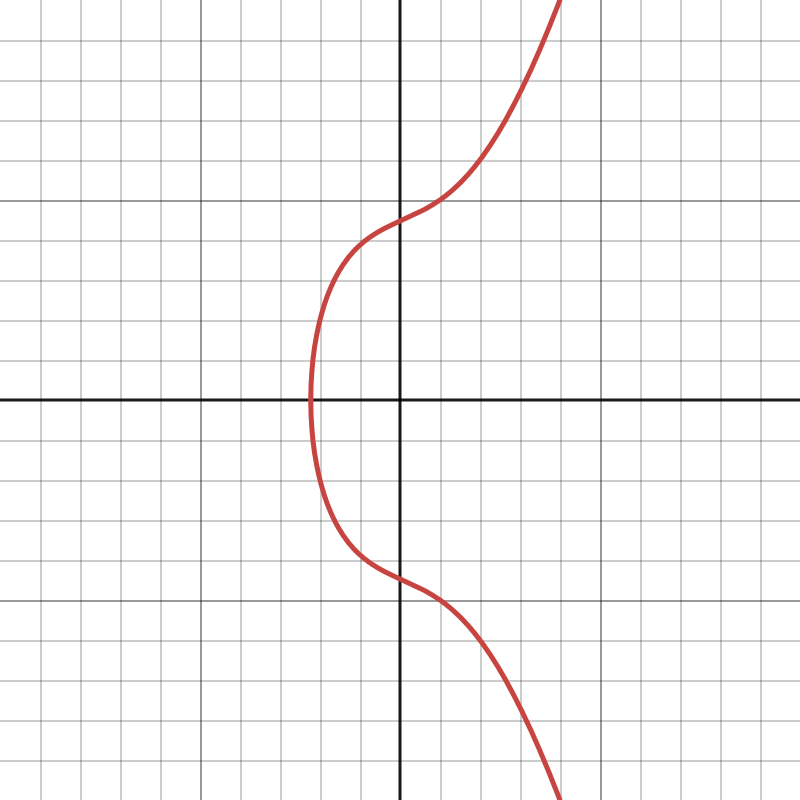
\includegraphics[width=0.3\linewidth]{images/finite-graph.png}
    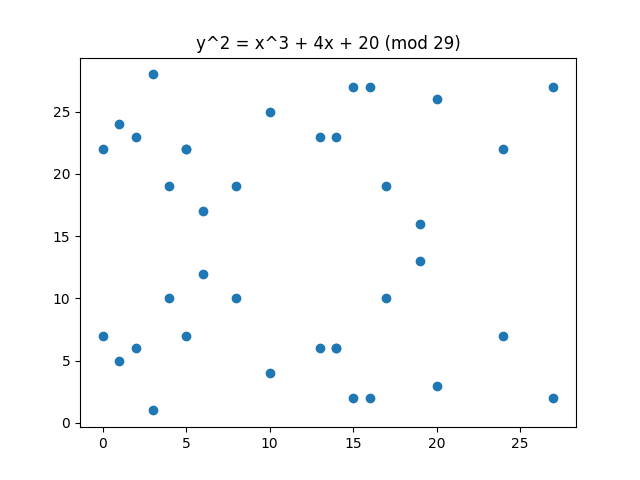
\includegraphics[width=0.4\linewidth]{images/finite-plt.png}
    \caption{$y^2=x^3+4x+20$ over $\mathbb{R}$ and $\mathbb{Z}_{29}$}
    \label{fig:finite}
\end{figure}

\subsection{Cyclical groups \& subgroups}


\section{Public key cryptography with elliptic curves}

\subsection{Point multiplication}

\subsection{Elliptic Curve Diffie-Hellman (ECDH)}


\newpage
\bibliographystyle{jox}
\bibliography{bibliography}

\end{document}